\section{Real-world experiments}\label{real_world_experiments}
This section describes the experiments performed using the prototype in a real-world scenario performing a distributed MapReduce computation on distributed heterogeneous devices.

\subsection{Computation}
The operation chosen for the experiment is a basic classification based on the distance from centroids, each representing its corresponding class:
\begin{itemize}
    \item \textbf{Red centroid}: (200,900)
    \item \textbf{Green centroid} (700,100)
    \item \textbf{Blue centroid} (1300,700)
\end{itemize}

\begin{figure}[!ht]
    \centering
    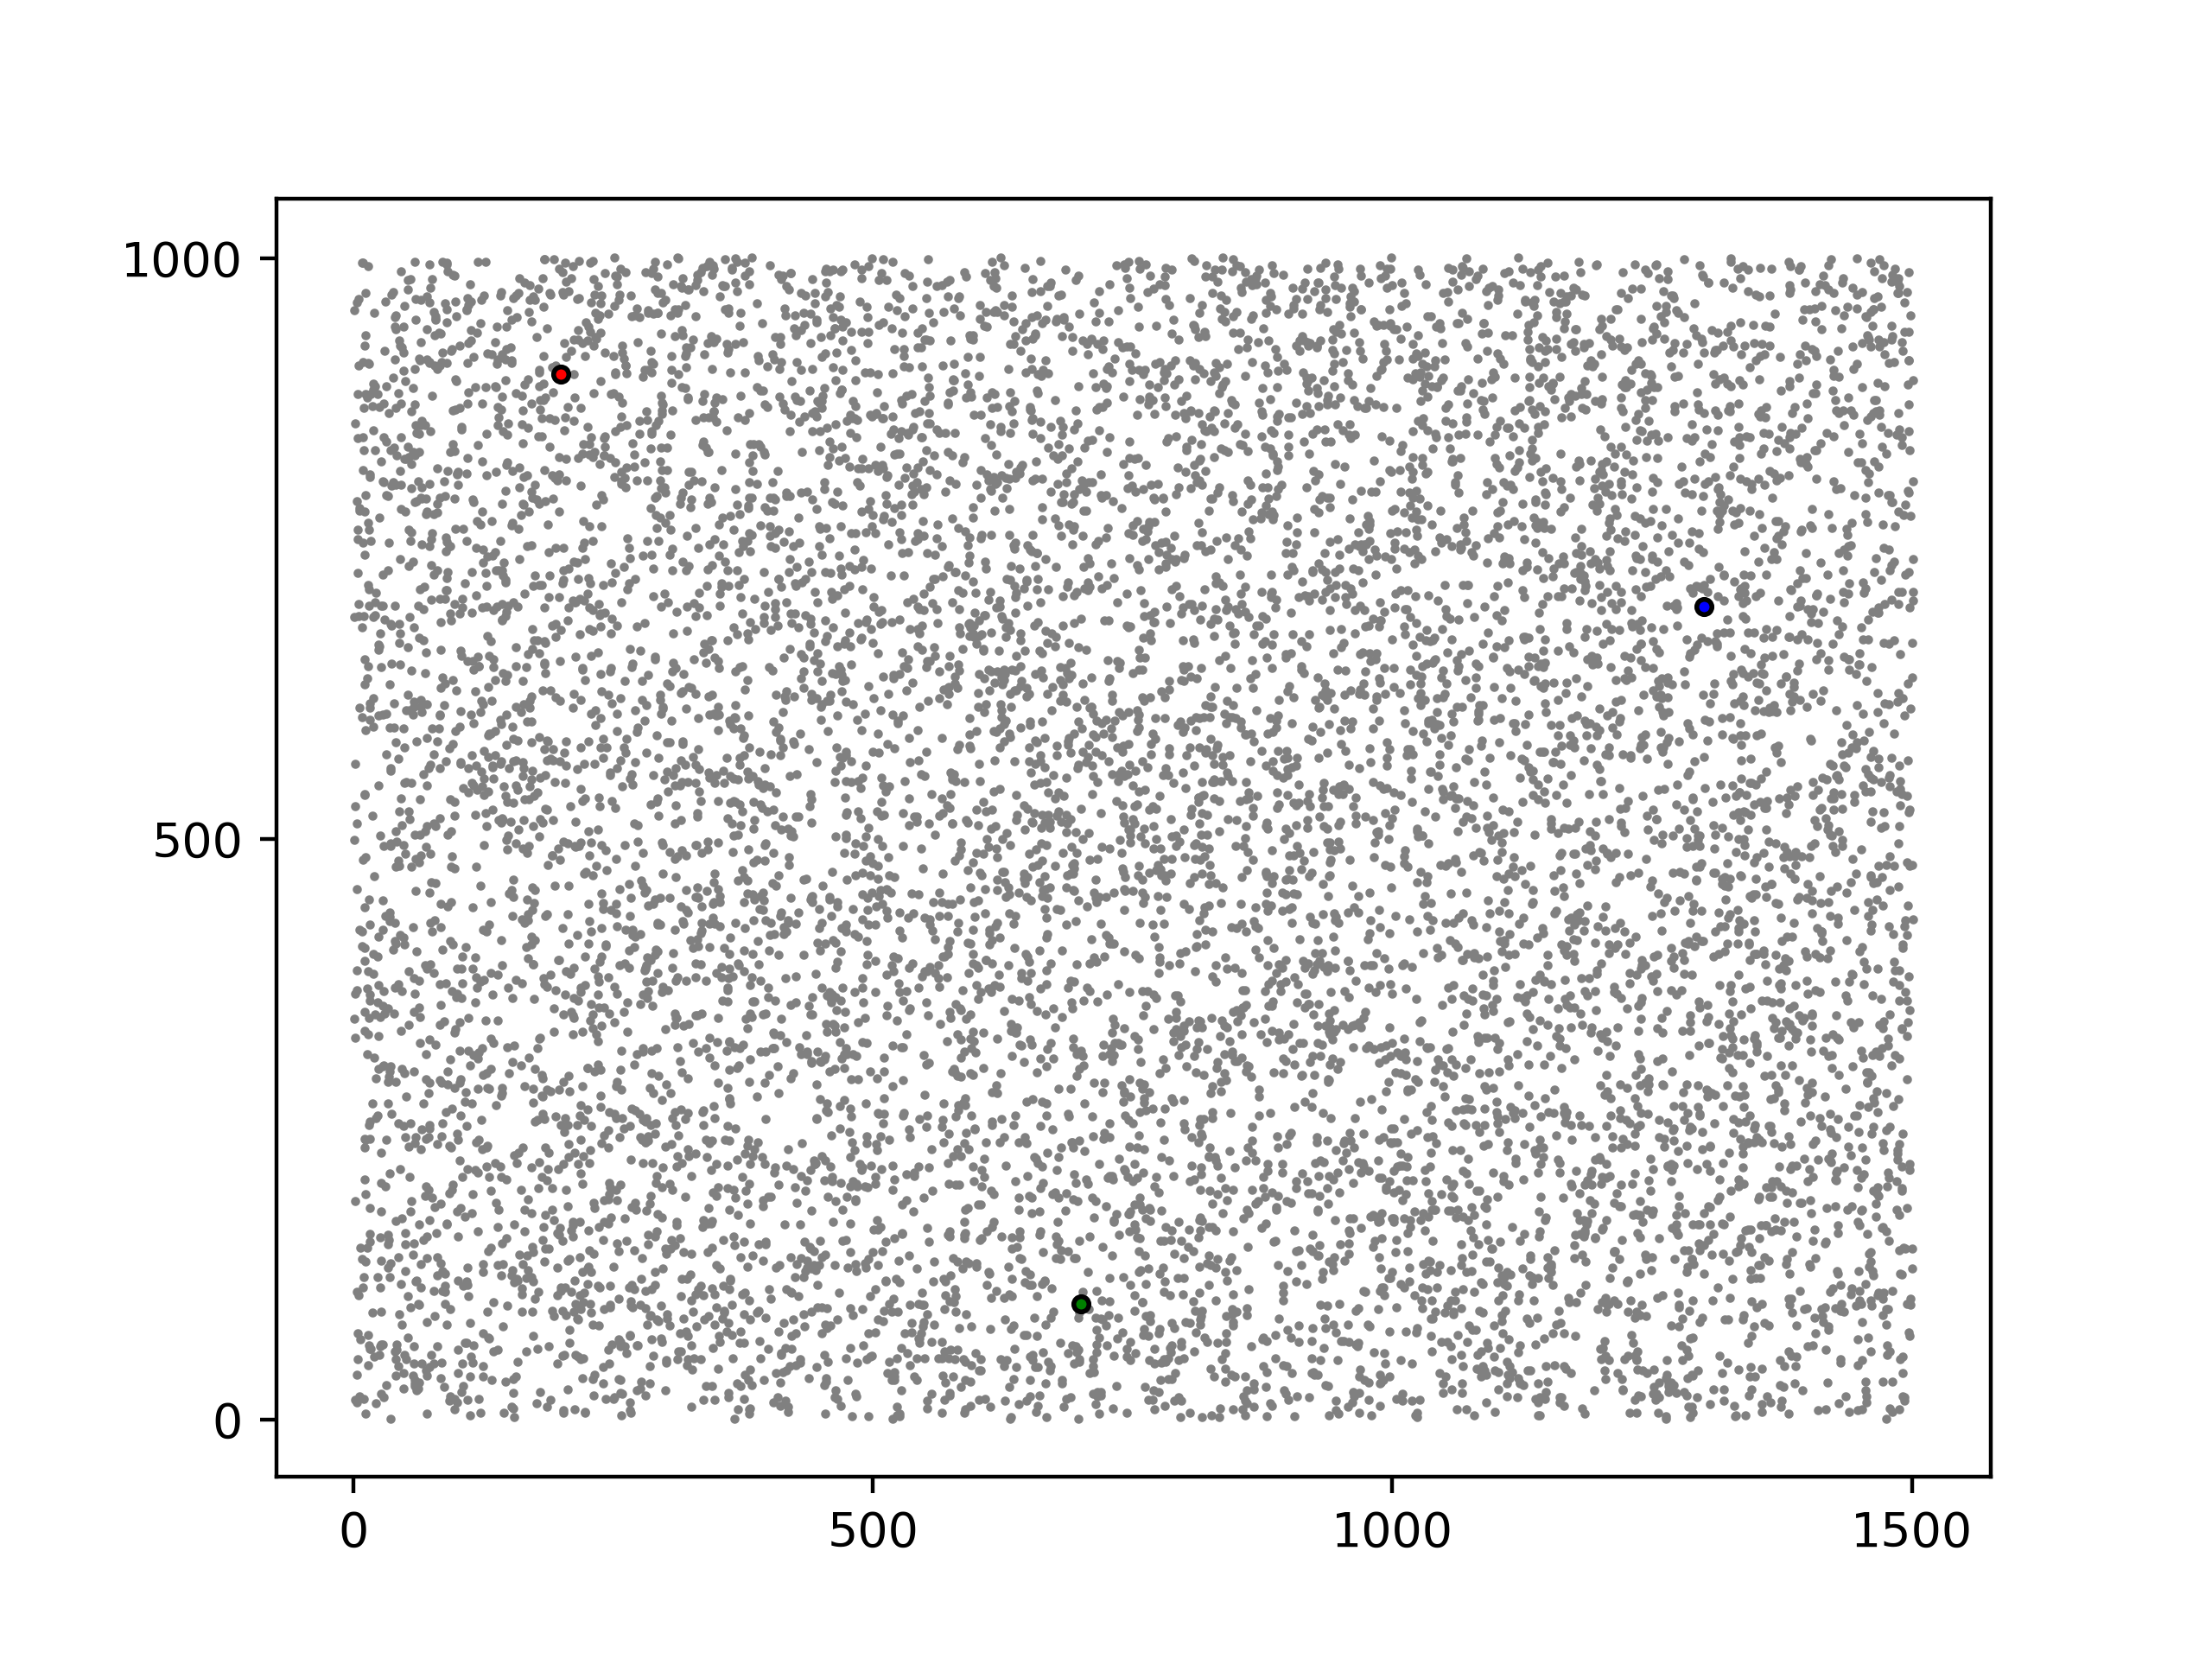
\includegraphics[width=\linewidth]{document/chapters/chapter_7/images/computation_start.png}
    \caption{Computation - Starting point}
    \label{fig:computation_start}
\end{figure}

Given a Cartesian plane (width: [0,1500], height: [0, 1000]) and a set of 2D points contained in it, the map function takes as input one of said points and calculates the euclidean distance from each one of the centroids; the centroid with minimum distance among the three is then chosen, obtaining a key-value output composed by the chosen class as the key and an array containing the computed point as the value (the array becomes relevant in the reduce function). It is important to note that in comparing the distance among two points, the square root characterizing the euclidean distance is not needed and, therefore, it is not calculated in the map function.

\begin{lstlisting}
const mapFunction = (p) => {
    const x = p[0];
    const y = p[1];
    const red = Math.pow(x - 200, 2) + Math.pow(y - 900, 2);
    const green = Math.pow(x - 700, 2) + Math.pow(y - 100, 2);
    const blue = Math.pow(x - 1300, 2) + Math.pow(y - 700, 2);
    switch(Math.min(red, green, blue)){
        case red: return ["red", [p]];
        case green: return ["green", [p]];
        case blue: return ["blue", [p]];
    }
}
\end{lstlisting}

Every data region is computed by the Map Workers and, after every point in a particular region is classified, the output (visualized in \textit{figure \ref{fig:computation_region_computation}}) can be computed in the reduce function which simply reunites the intermediate results with the same key (hence belonging to the same class) in a single array.

\begin{lstlisting}
const reduceFunction = (p1, p2) => {
    p1.push(p2[0]);
    return p1;
}
\end{lstlisting}

\begin{figure}[!ht]
    \centering
    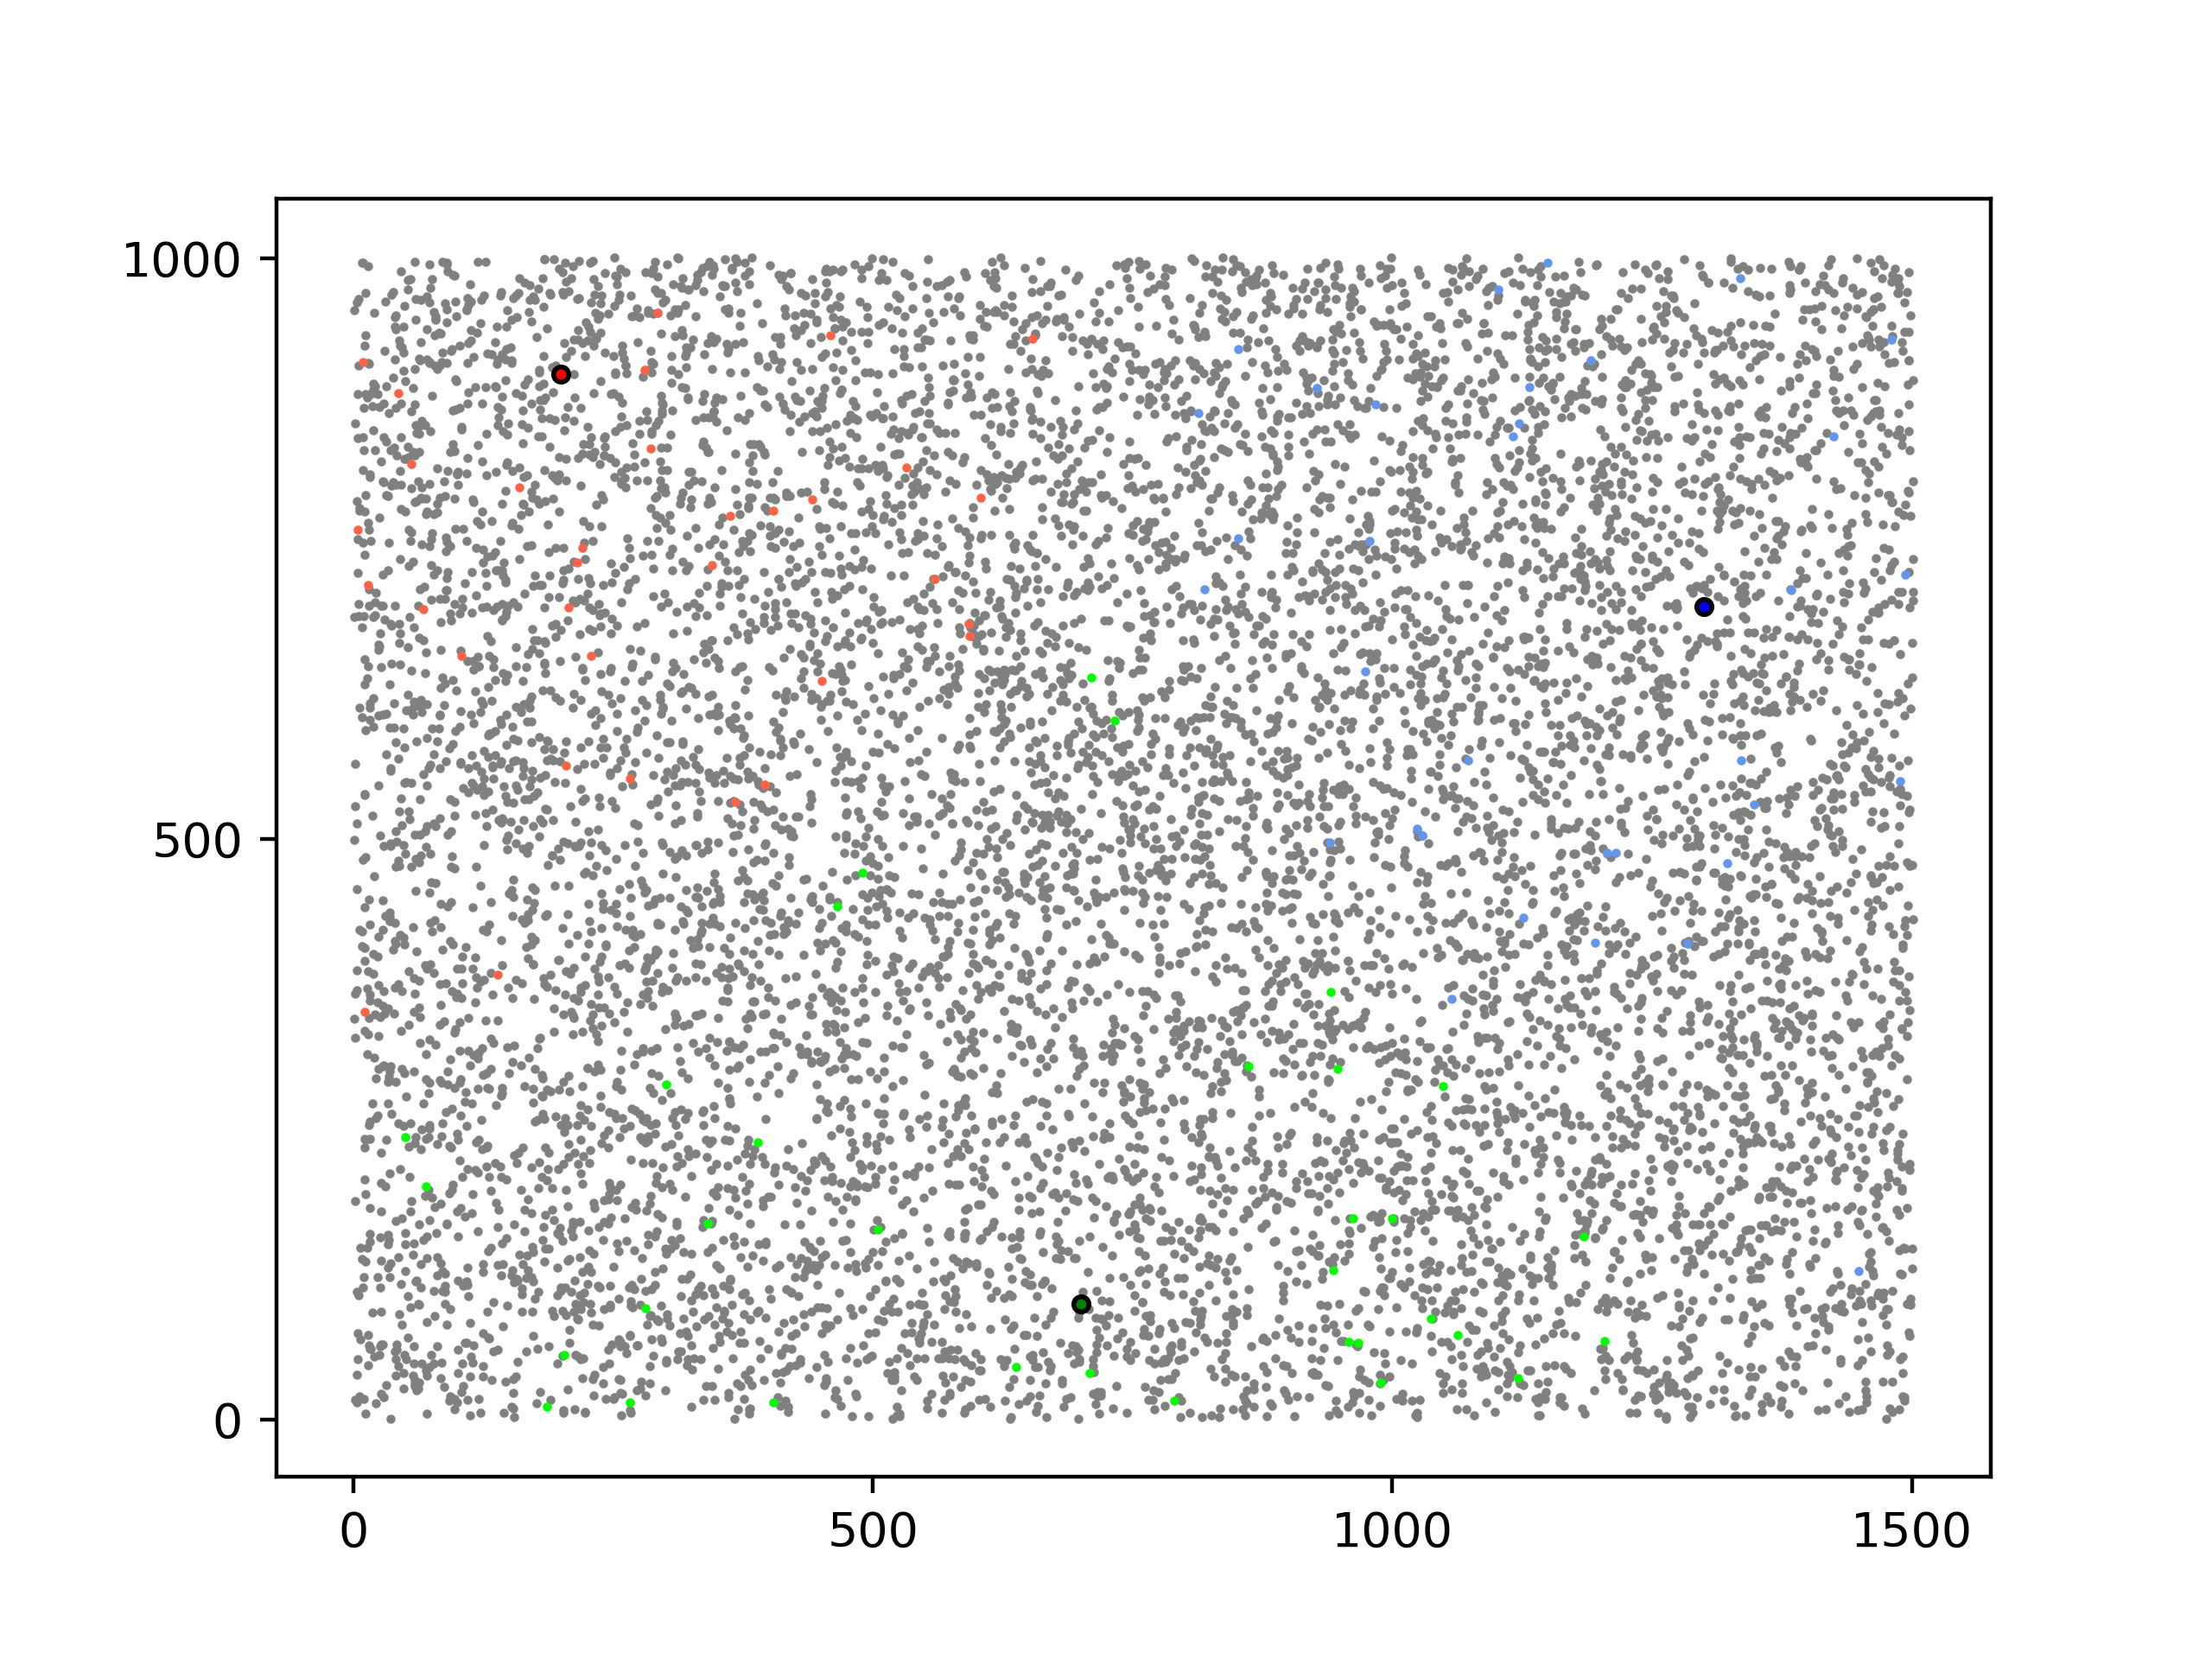
\includegraphics[width=\linewidth]{document/chapters/chapter_7/images/computation_region_computation.png}
    \caption{Computation - Region computation}
    \label{fig:computation_region_computation}
\end{figure}

As can be seen in \textit{figure \ref{fig:computation_final_result}}, after every region is mapped and then reduced, each point is assigned to one of the three classes.

\begin{figure}[!ht]
    \centering
    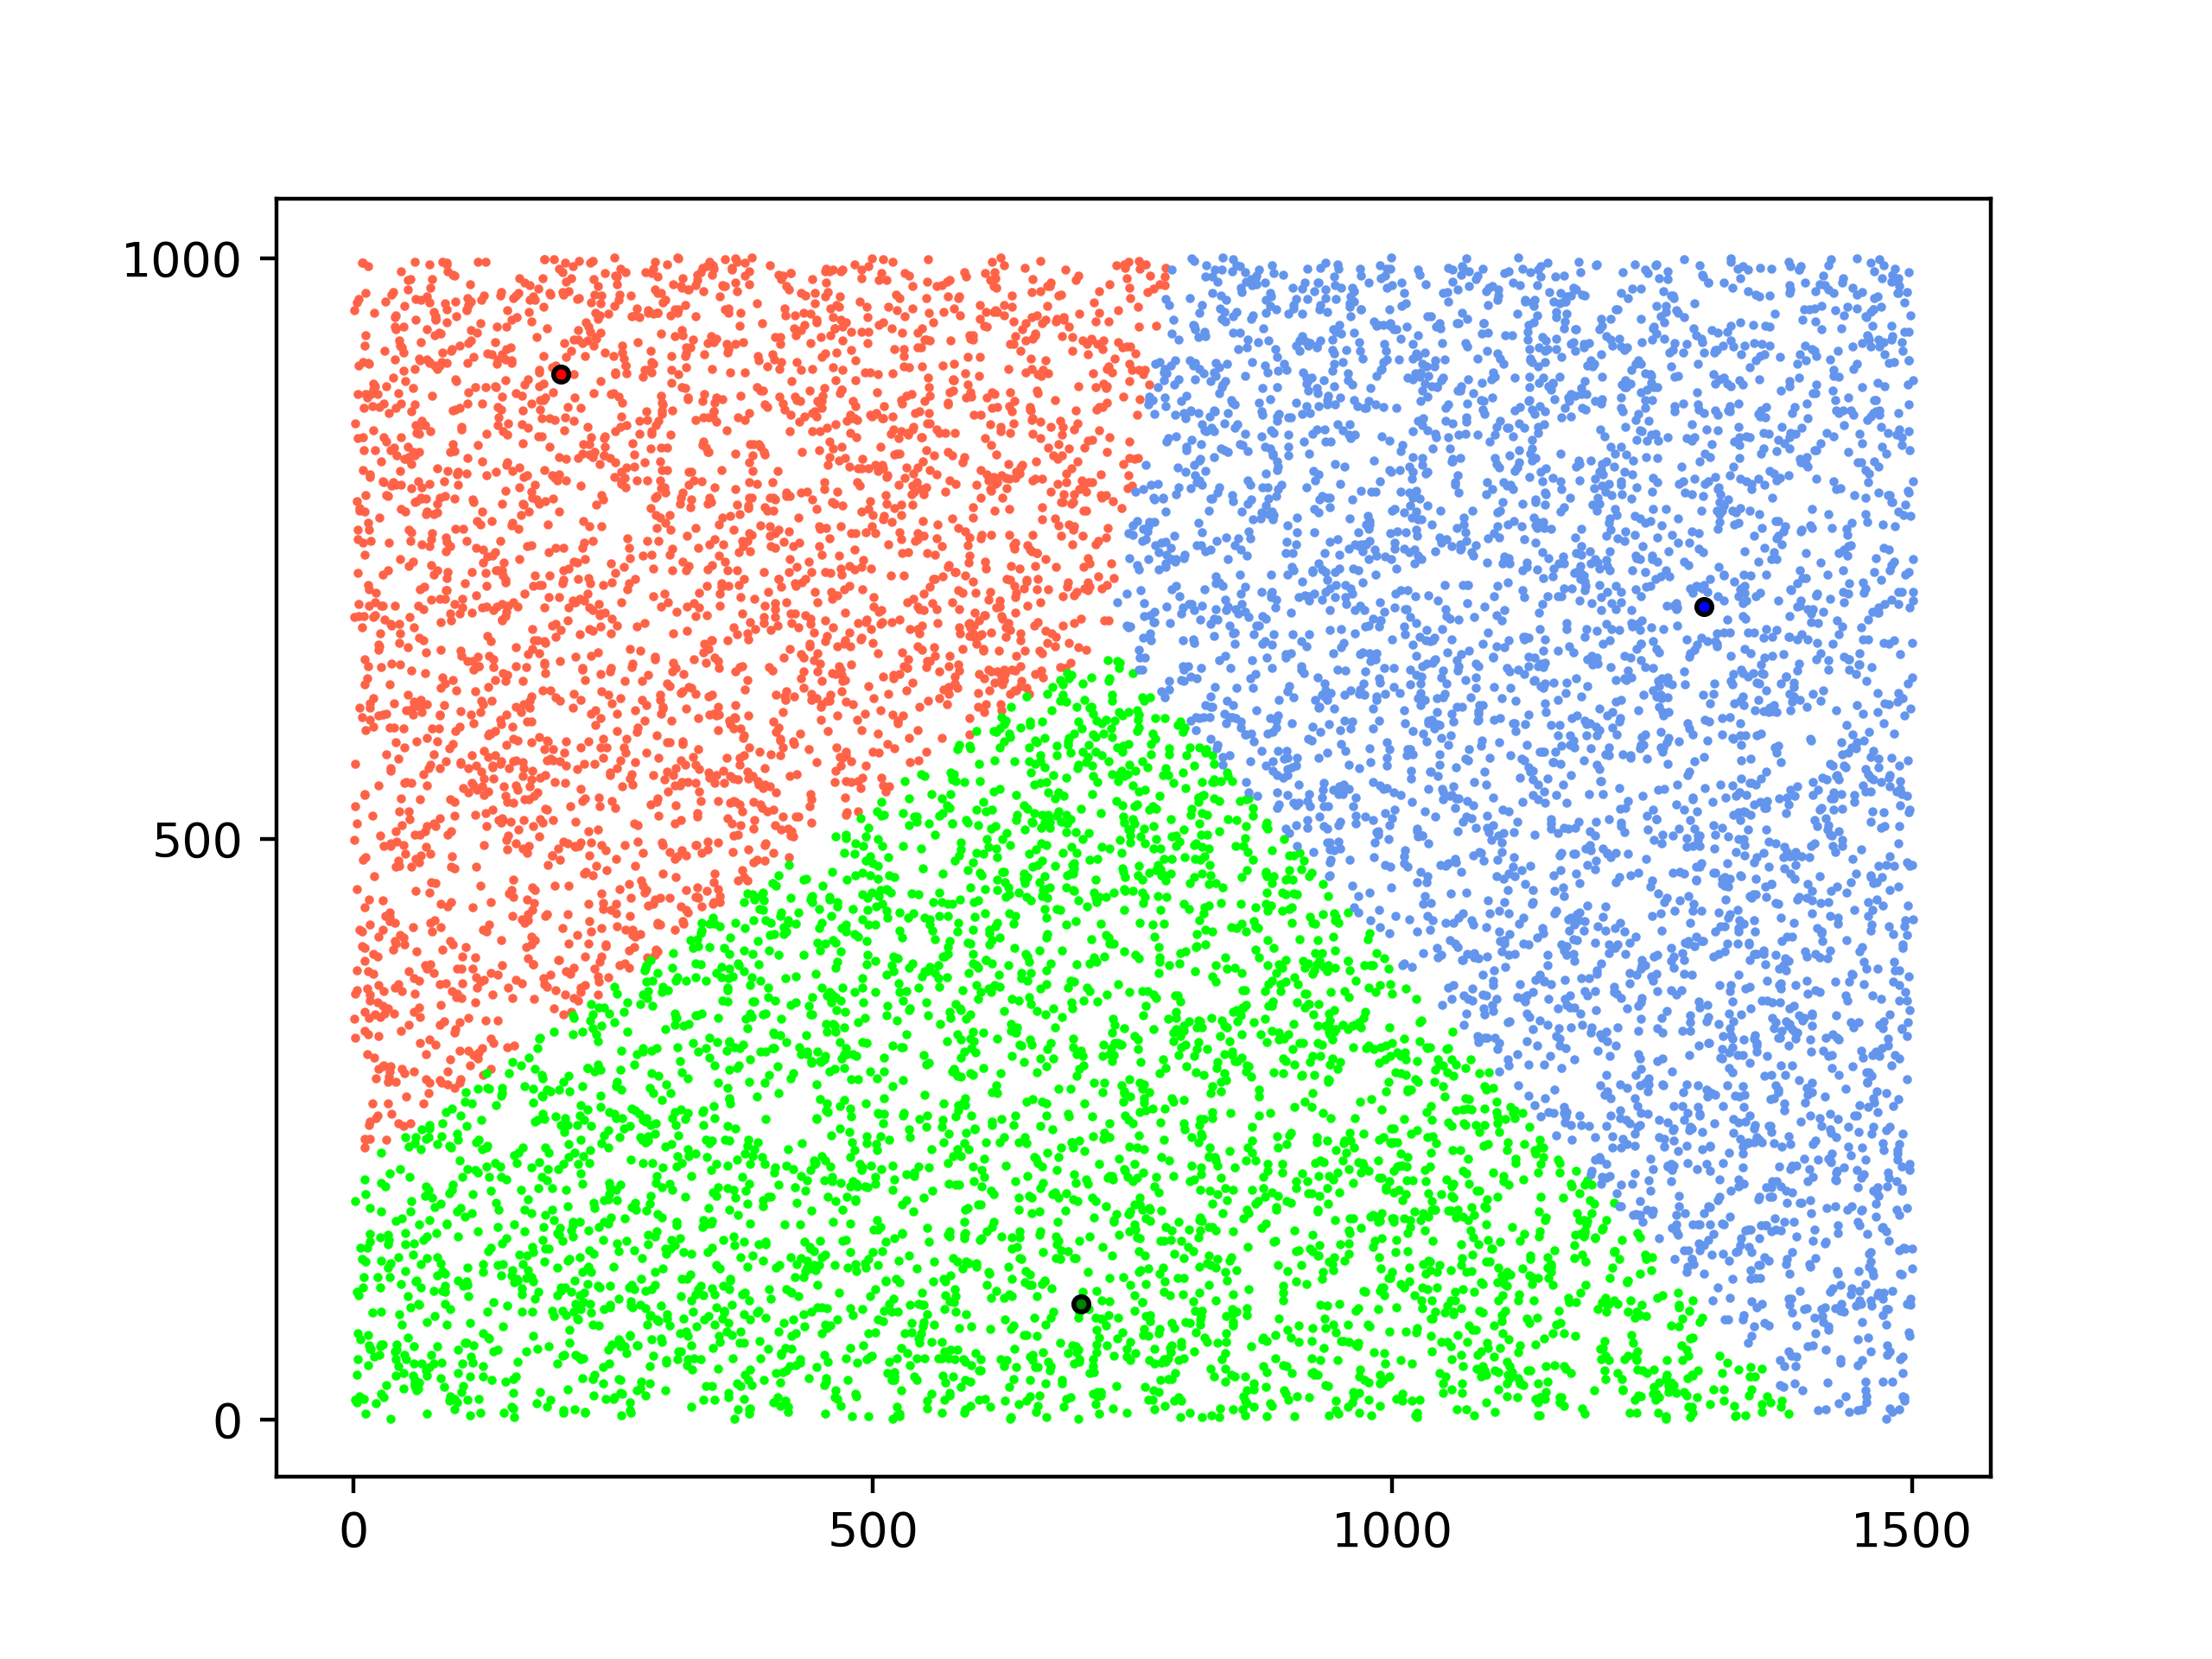
\includegraphics[width=\linewidth]{document/chapters/chapter_7/images/computation_final_result.png}
    \caption{Computation - Final result}
    \label{fig:computation_final_result}
\end{figure}

\subsection{Setup}

\begin{figure}[!ht]
    \centering
    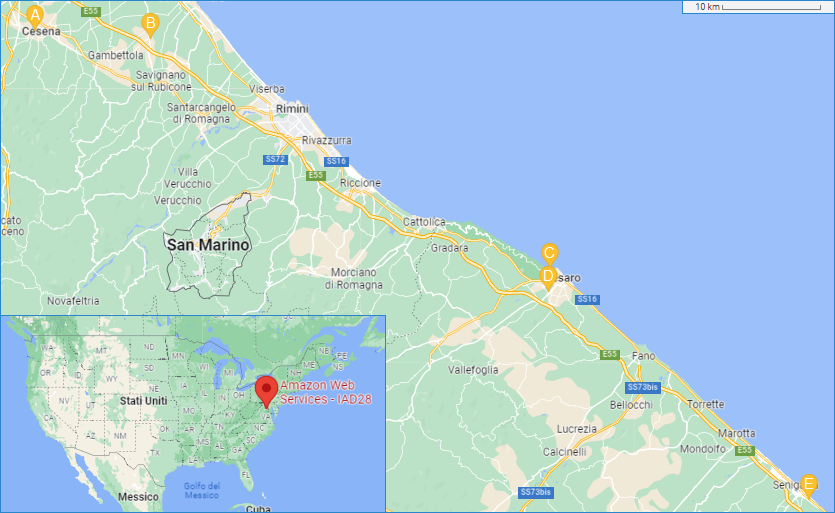
\includegraphics[width=\linewidth]{document/chapters/chapter_7/images/experiment_devices_setup.png}
    \caption{Devices setup}
    \label{fig:experiment_devices_setup}
\end{figure}

\subsection{Results}
TODO

\begin{figure}[!ht]
    \centering
    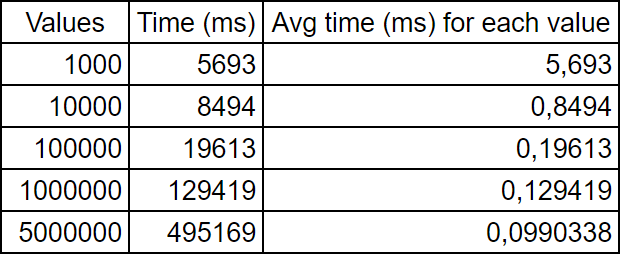
\includegraphics[scale=0.55]{document/chapters/chapter_7/images/experiment_results.png}
    \caption{Experiment results}
    \label{fig:experiment_results}
\end{figure}

\begin{figure}[!ht]
    \centering
    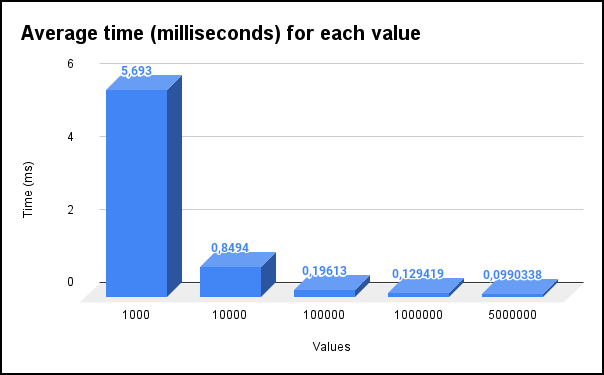
\includegraphics[scale=0.55]{document/chapters/chapter_7/images/experiment_results_avg_ms_per_value.png}
    \caption{Average time (milliseconds) for each value}
    \label{fig:experiment_results_avg_ms_per_value}
\end{figure}